%----------------------------------------------------------------------------------------

%\documentclass[paper=a4, fontsize=11pt]{scrartcl} % A4 paper and 11pt font size
\documentclass[11pt,twocolumn]{article}

\usepackage[T1]{fontenc} % Use 8-bit encoding that has 256 glyphs
%\usepackage{fourier} % Use the Adobe Utopia font for the document - comment this line to return to the LaTeX default
\usepackage[english]{babel} % English language/hyphenation
\usepackage{amsmath,amsfonts,amsthm} % Math packages
\usepackage{mathtools}
\usepackage{lipsum} % Used for inserting dummy 'Lorem ipsum' text into the template
\usepackage[margin=2.5cm]{geometry}
\usepackage{xcolor}
\usepackage{listings}
\usepackage{url}
\usepackage{mdframed}
\usepackage{graphicx}
\usepackage{caption}
\usepackage{natbib}

\usepackage{sectsty} % Allows customizing section commands
\allsectionsfont{\centering \normalfont\scshape} % Make all sections centered, the default font and small caps

\usepackage{fancyhdr} % Custom headers and footers
\pagestyle{fancyplain} % Makes all pages in the document conform to the custom headers and footers
\fancyhead{} % No page header - if you want one, create it in the same way as the footers below
\fancyfoot[L]{} % Empty left footer
\fancyfoot[C]{} % Empty center footer
\fancyfoot[R]{\thepage} % Page numbering for right footer
\renewcommand{\headrulewidth}{0pt} % Remove header underlines
\renewcommand{\footrulewidth}{0pt} % Remove footer underlines
\setlength{\headheight}{15.0pt} % Customize the height of the header

\numberwithin{equation}{section} % Number equations within sections (i.e. 1.1, 1.2, 2.1, 2.2 instead of 1, 2, 3, 4)
\numberwithin{figure}{section} % Number figures within sections (i.e. 1.1, 1.2, 2.1, 2.2 instead of 1, 2, 3, 4)
\numberwithin{table}{section} % Number tables within sections (i.e. 1.1, 1.2, 2.1, 2.2 instead of 1, 2, 3, 4)

\setlength\parindent{20pt} % Removes all indentation from paragraphs - comment this line for an assignment with lots of text

\newcommand{\vect}[1]{\mathbf{#1}}
\newcommand{\params}{\boldsymbol{\theta}}
\newcommand{\dn}[1]{\partial{#1}}

%----------------------------------------------------------------------------------------
%	TITLE SECTION
%----------------------------------------------------------------------------------------

\newcommand{\horrule}[1]{\rule{\linewidth}{#1}} % Create horizontal rule command with 1 argument of height

\title{	
\normalfont \normalsize 
\textsc{Department Of Computer Science, University of Bath} \\ [5pt] % Your university, school and/or department name(s)
\textsc{EngD in Digital Entertainment} \\ [5pt] 
\horrule{0.7pt} \\[0.2cm] % Thin top horizontal rule
\Huge A review on crowd simulation and rendering \\ % The assignment title
\vspace{7 mm}
\Large CM50244 \: Computer Animation and Games I \\
\horrule{0.7pt} \\[0.0cm] % Thick bottom horizontal rule
}
\author{Garoe Dorta-Perez \\ \Large Unit Leader: Prof Phil Willis \\}  % Your name\\ 

\begin{document}
\vspace*{\fill}
\begin{center}
\begin{minipage}{1.0\textwidth}

\clearpage\maketitle % Print the title
\thispagestyle{empty}

\end{minipage}
\end{center}
\vfill
\clearpage
\setcounter{page}{1}

%% Required for all content. 

% IMPORTANT
% ------------------------------------
% HAS TO has 2000 words
% ------------------------------------

\section{Introduction}

%Include why crowd simulation is interesting in films and videogames????
Crowds are encountered frequently, be it a large number of people in big shopping area, on a popular sports event, or at a demonstration.
While also other types of crowds are also common, such as schools of fish or flocks of birds.
While motives for simulating them range from: \textit{film industry} where it is not always possible or economically viable to have a real crowd,also in \textit{video games} as the game world might have need for a crowd, including \textit{disaster prevention and management} where they are used to aid in the decision making process as they provided a new source of data.

A crowd is much more than the collections of individuals that form it.
And as such the behaviour of the individuals could be affected by other members of the crowd.
History shows how in some cases crowd of people behave in a well organized manner, while in others its individual act selfishly abandoning all social norms.
When simulating this interactions with a naive approach, as the numbers of individuals in the crowd increase the computational cost of the interrelations calculation increments exponentially.

This problem has actually a number of clearly differentiated areas.
Firstly there is a \textit{crowd generation} problem, a modeller needs user-friendly tools in order to set up a scene in which a crowd is present.
Secondly the crowd is an evolving entity, so a \textit{crowd dynamics model} is required to govern the state of the crowd over time.
Thirdly, the model should be presented to the user, so a \textit{rendering} stage is needed.

Crowd simulation and rendering has been an active research area as early as 1987 with the work on birds flocks by \cite{Reynolds1987}.
There, he proved that by implementing some local rules in each entity a coherent global behaviour could be achieved.

\section{Classification}

A clear line can be drawn between real-time simulation (games) and non real-time simulation (films).
Since the requirements for each simulation are quite different and so are the techniques used in each area.

\subsection{Modelling Classifications}

In order to simulate crowd behaviour a number of approaches have been proposed.
As they shared certain similarities they can be divided using a common criteria such as time of the simulation and size of the modelled crowd.
Regarding time, we have short-term simulations, medium-term simulations and long-term simulations.
While in terms of size a distinction can be made among small, medium and big size crowds.
We can also use as criteria the type of model used for the agents in the crowd, either \textbf{entity based}, all individuals are homogeneous, or \textbf{agent based}, each individual is intelligent and autonomous.

Generally, agent based or entity based systems are used for small and medium crowds.
Due to the challenging nature of big size crowds the most common approach is to adopt a \textbf{flow based} simulation.

\subsection{Rendering Classifications}

The different types of rendering techniques can be classified in the following groups: 
\textbf{dynamically generated impostors}, this procedure involves displaying 2D billboards with fixed poses instead of the full model,~\cite{Aubel2000}.
\textbf{Point-rendering} techniques build multi-resolution representations using point samples from the mesh,~\cite{Wand2002}.
\textbf{Dynamic meshes} take advantage of the shaders pipeline to dynamically render humans with a variety of colors, animation and appearance,~\cite{Ciechomski2005}.

\section{Generating crowds}

Before the crowd can be simulated or rendered it has to be generated.
This task is usually has not been research as deeply as the rest.
This step essentially involves setting the initial parameters at which the crowd operates.

\cite{Ulicny2004} proposed a brush metaphor to manipulate crowds.
His technique allows the user select an brush operator(create individuals, change color, etc) and apply it in the crowd world space.
Altered individuals in the crowd will be those in sight in the screen domain.
Therefore an intuitive approach, as it is similar to what users as used to, is provided.
However it has certain limitations, such as lack of direct control over crowd behaviour or difficulty to select individuals in cluttered environments.

Some of the challenges were met by \cite{Jordao2014}, whose method introduces the concept of crowd patches.
Such areas allow the user to control the crowd through a sculpting metaphor.
While also addressing the problem of populating vast empty areas efficiently.
High level control of the motion is provided as the patches are editable in real time.
%Or the high level of control is provided through to uses of patches????

GIVE DRAWBACKS OF THIS PAPER

\section{Simulating crowds}

Give a short overview of each paper and what is important and how it evolves

\subsection{Agent Based}

aa

\subsection{Entity based Based}

aa

\subsection{Flow Based}

aa

\section{Rendering crowds}

How to achieve color variety

Height change

Accessories 

Animation variety

LOOK AT Challenges in Crowd Simulation paper to fill this in

\subsection{Dynamically Generated Impostors}
\subsection{Point-Rendering}
\subsection{Dynamic Meshes}

\section{Mayor milestones}

With the advent of programmable GPU there has been a shift of general computation from the CPU to the GPU with substantial increases in performance.

LOD techniques, impostors, mesh decimation, mesh subdivision, cloth simulation.

In order to lower the rendering cost ~\cite{pratt1997humans} TODO CHANGE TO CITED BY OTHER AUTHOR taken from ~\cite{Aubel1999} used a LOD technique to be able to render crowds, however even though it  achieved real time performance the realism of the models was quite poor.


%\begin{figure}[ht]
%  \centering
%  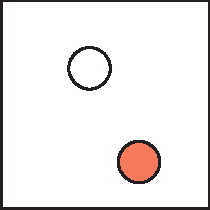
\includegraphics[width=1.5in]{images/samplefigure}
%  \caption{Sample illustration.}
%\end{figure}

\section{Conclusion}

%\bibliographystyle{acmsiggraph}
\bibliographystyle{apalike}
\bibliography{template}
\end{document}
